\chapter{WeMo Insight Switch Setup}
\label{ap: appendixC}

This appendix describes the steps required to connect the WeMo Switch to a WiFi network. A prerequisite requires downloading the Wemo app from Google Play or the Apple App Store. In order to initiate the connection process, the WeMo must be plugged into an outlet while holding down the the reset button for 5 seconds. This should allow the WeMo to broadcast its own WiFi network titled \say{WeMo.Insight.23A}. This WiFi network must be connected to allow the device to be paired with the desired network.

\section{Create a WeMo account}
If the app was recently downloaded, a screen shown in Figure~\ref{fig:signInWemo} is displayed where the user can either create an account or sign in with an existing account.
\begin{figure}[H]
\centering
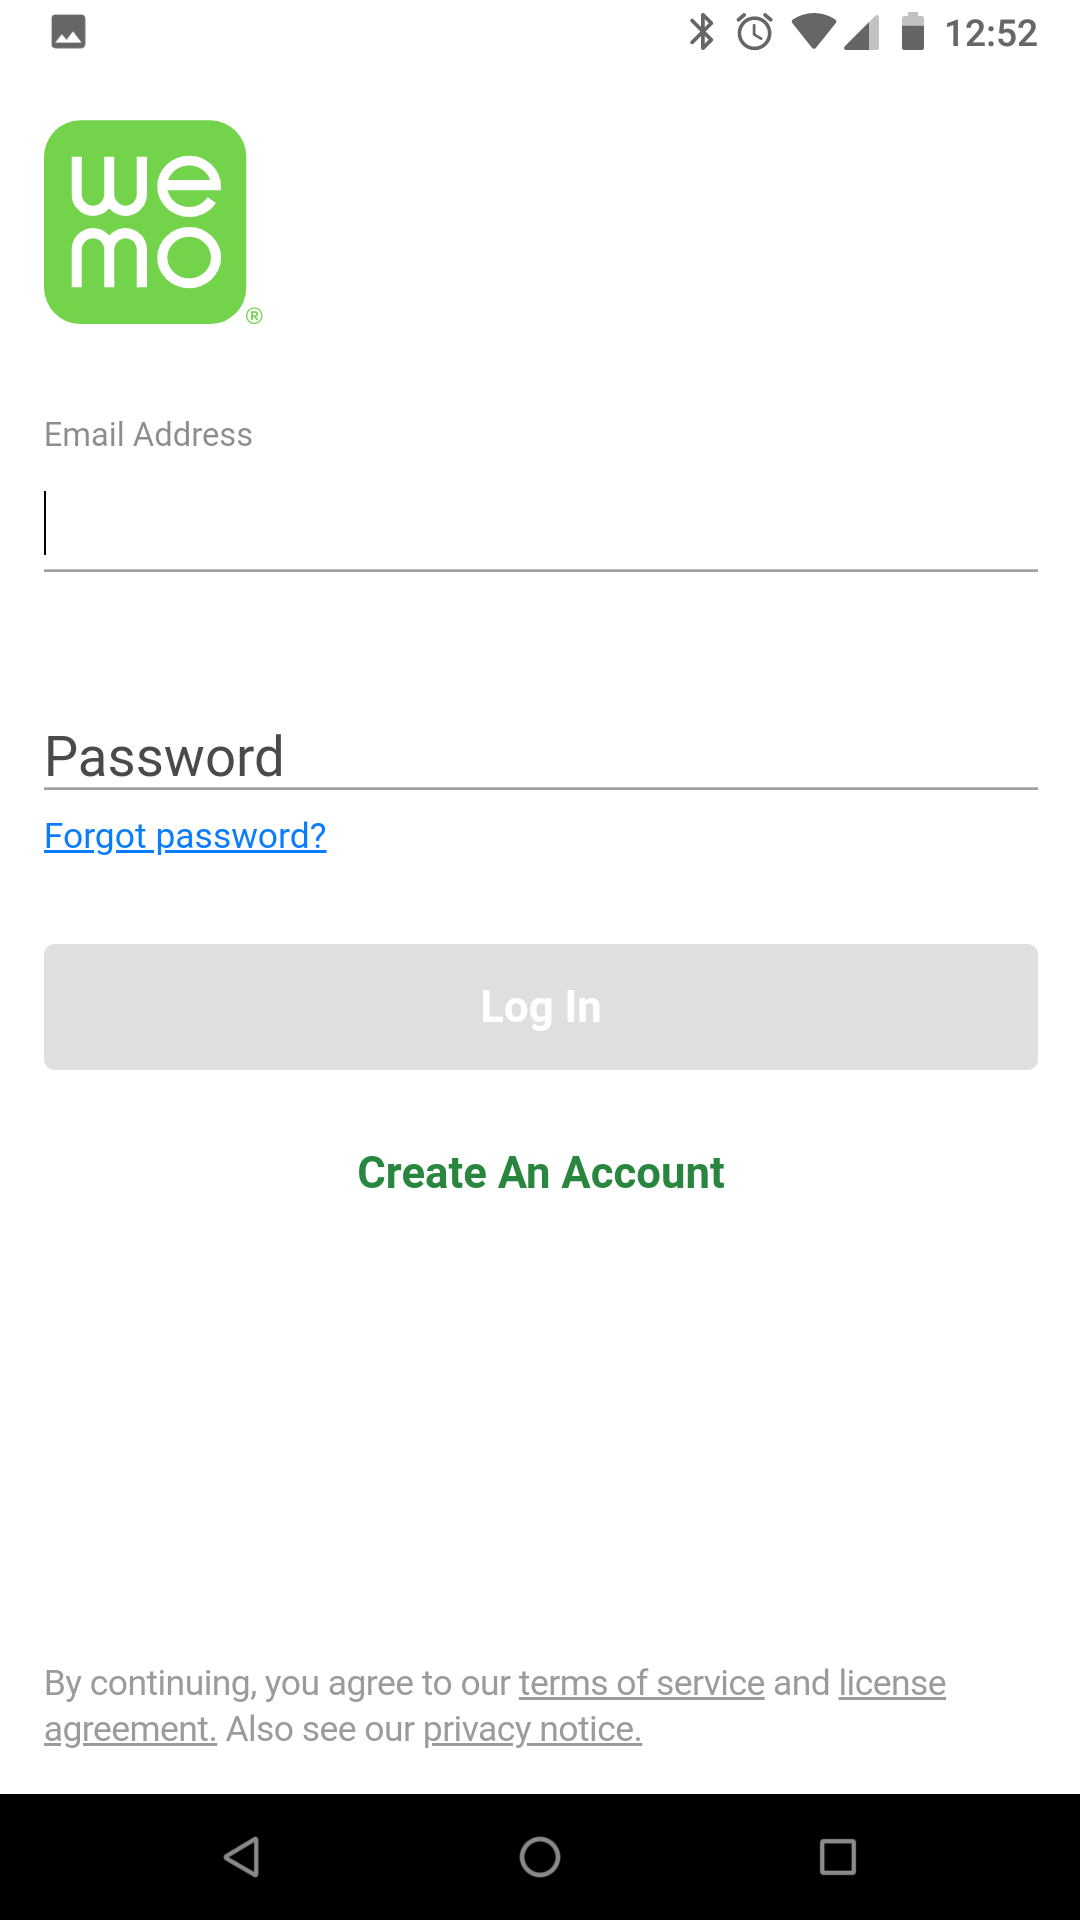
\includegraphics[scale=0.09]{figs/wemoApp/signInWemo.png}
\caption{WeMo app sign-in page}
\label{fig:signInWemo}
\end{figure}

\section{Name the device}
A screen will appear asking the user to enter the friendly name of the device as in Figure~\ref{fig:nameDevice}
\begin{figure}[H]
\centering
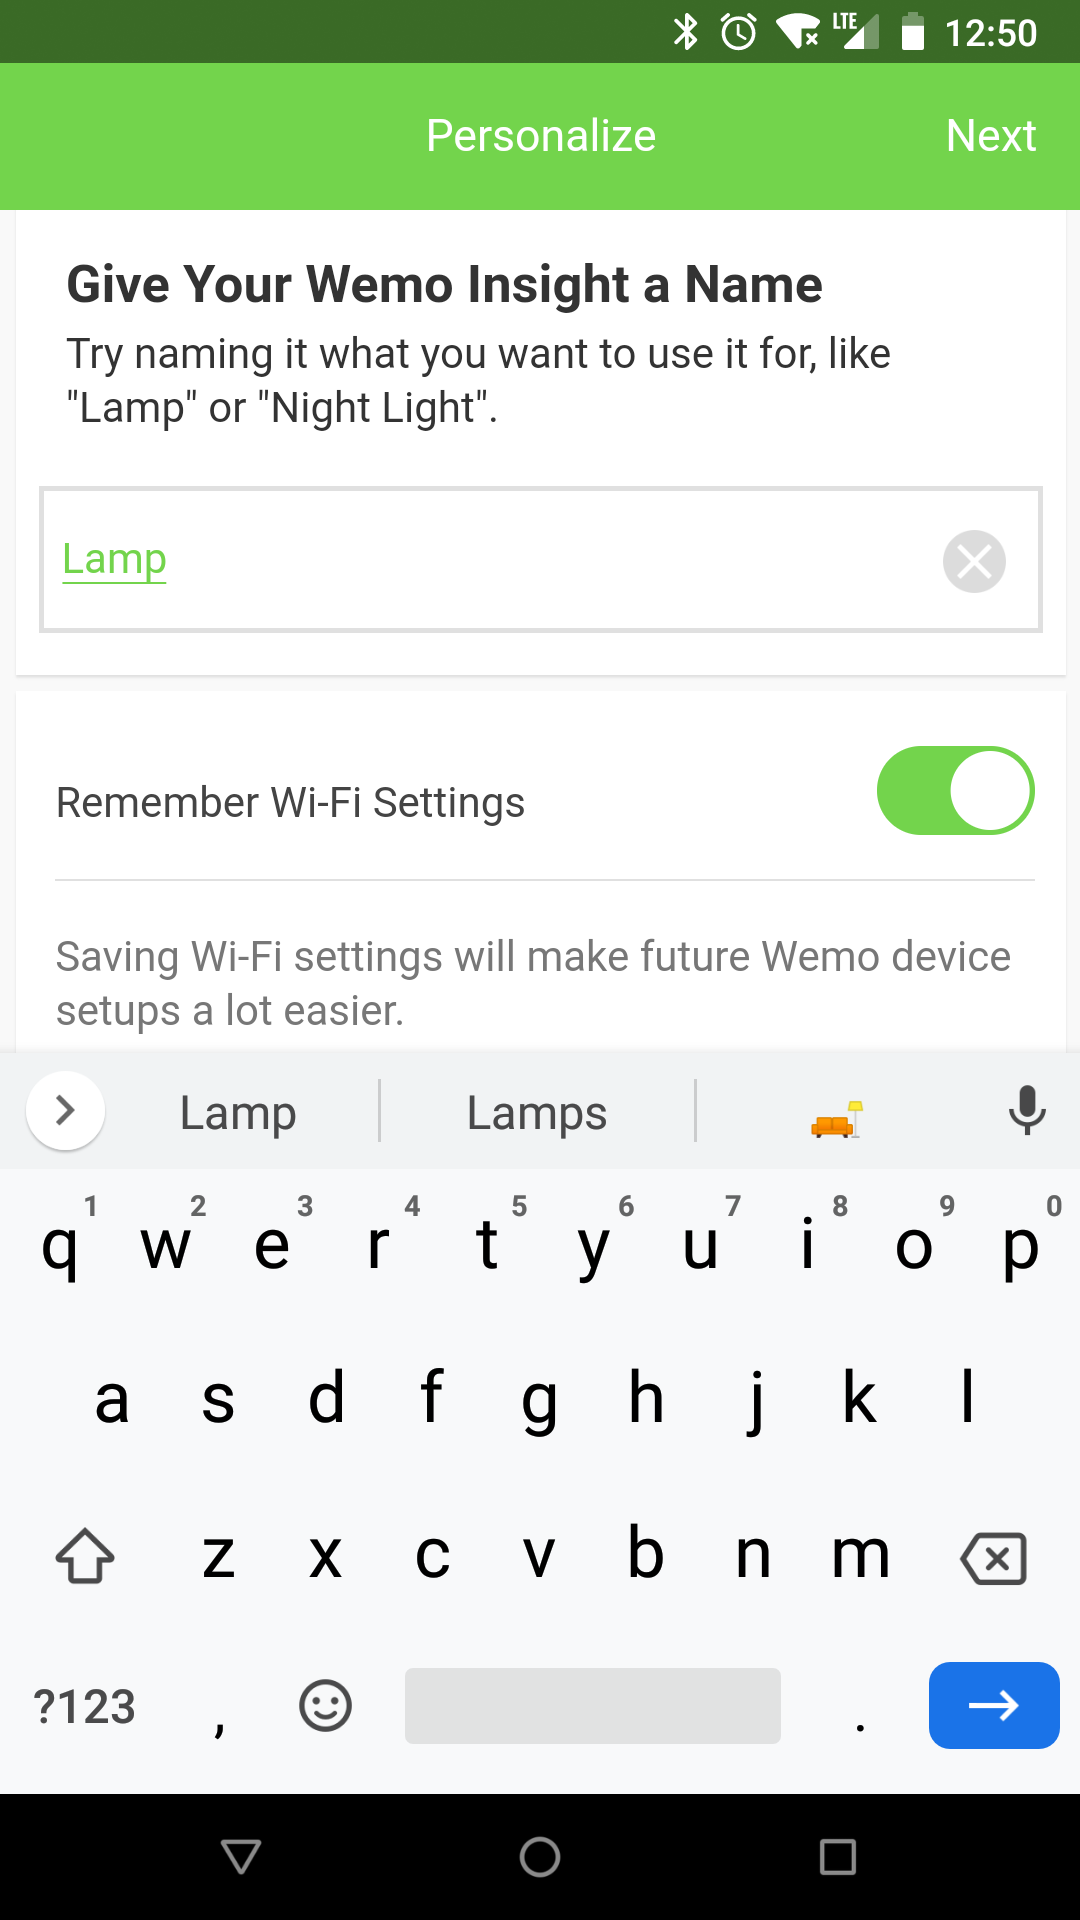
\includegraphics[scale=0.09]{figs/wemoApp/nameDevice.png}
\caption{Name device page}
\label{fig:nameDevice}
\end{figure}

\section{Pair WiFi network with the WeMo}
If the plug's WiFi network is connected to on the user's phone, the user will be prompted to connect to the desired WiFi network. Once this pairing is complete the screen in Figure~\ref{fig:completedSetup} will appear.
\begin{figure}[H]
\centering
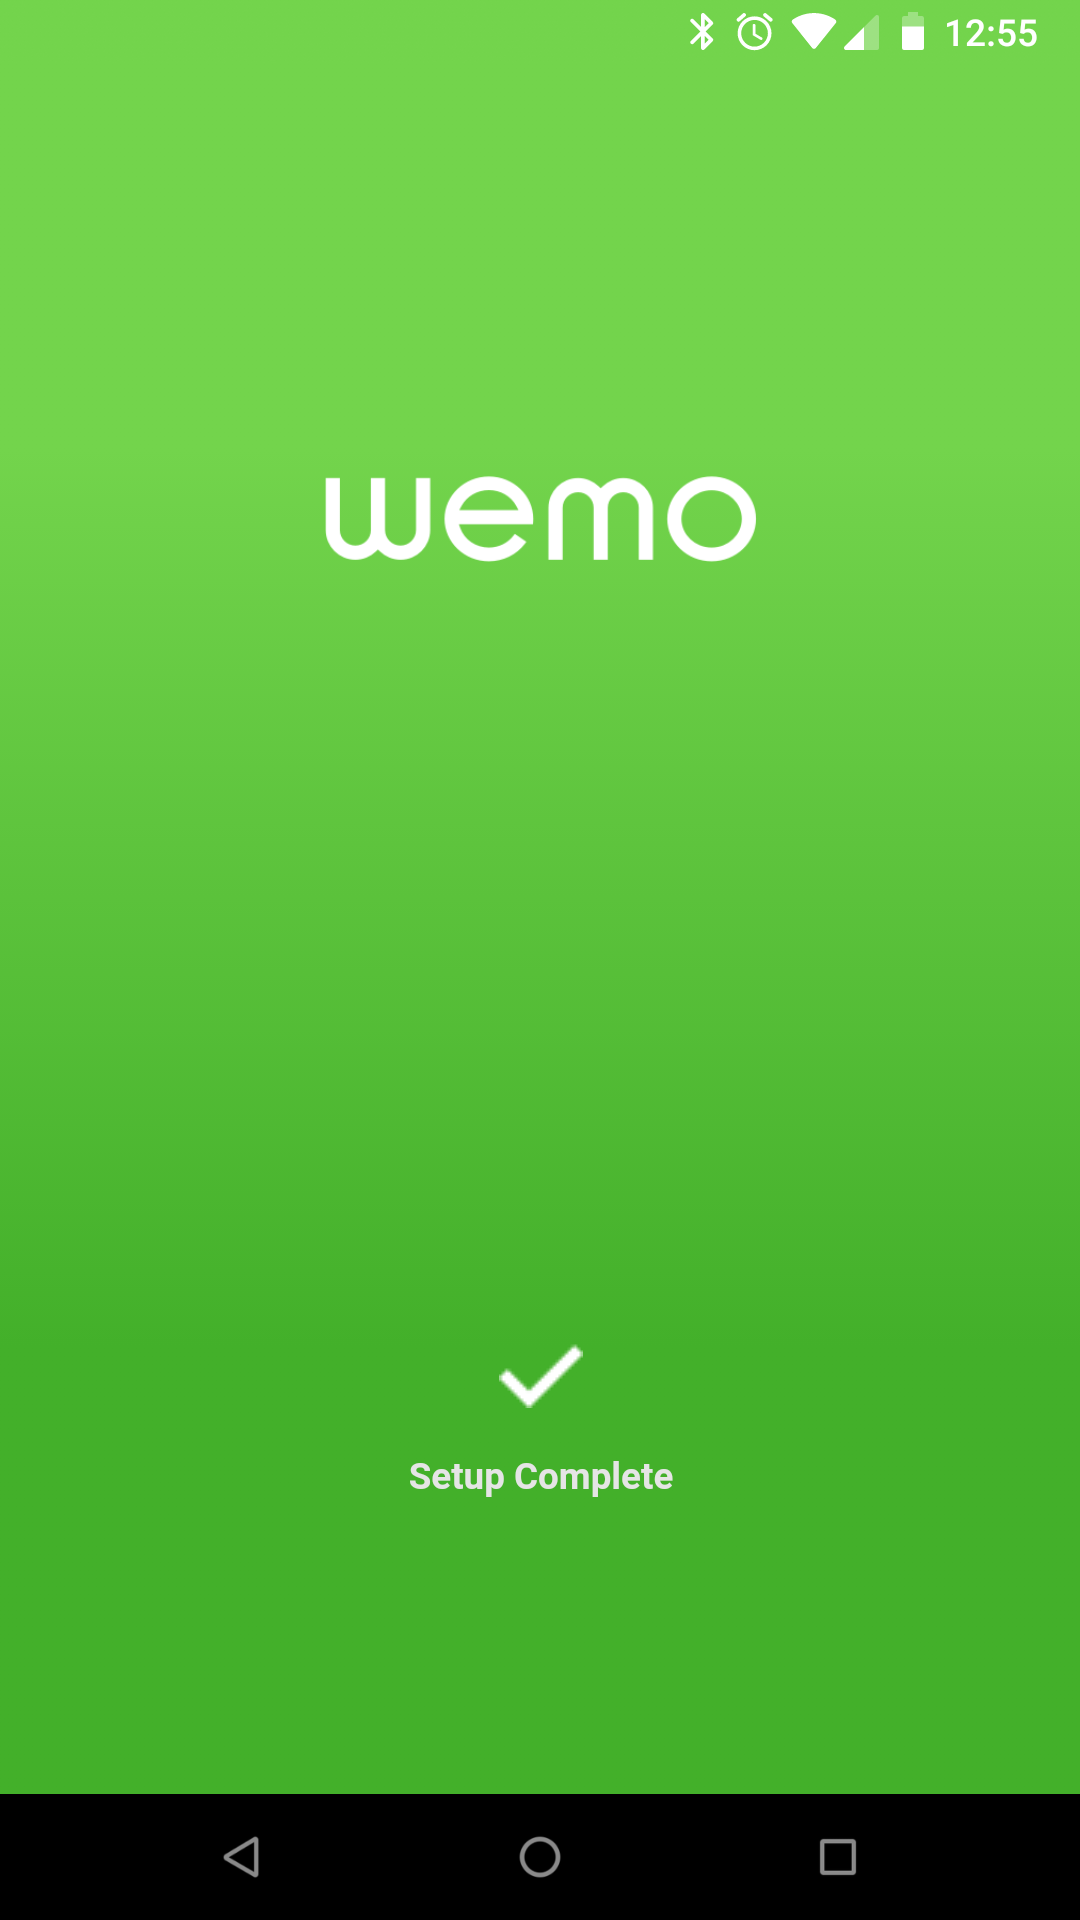
\includegraphics[scale=0.09]{figs/wemoApp/setupComplete.png}
\caption{Completed setup}
\label{fig:completedSetup}
\end{figure}

\section{Control the WeMo}
If everything was setup successfully, the user should be able to turn on and off the WeMo and see the power usage as in Figure~\ref{fig:smartPlutControl}.
\begin{figure}[H]
\centering
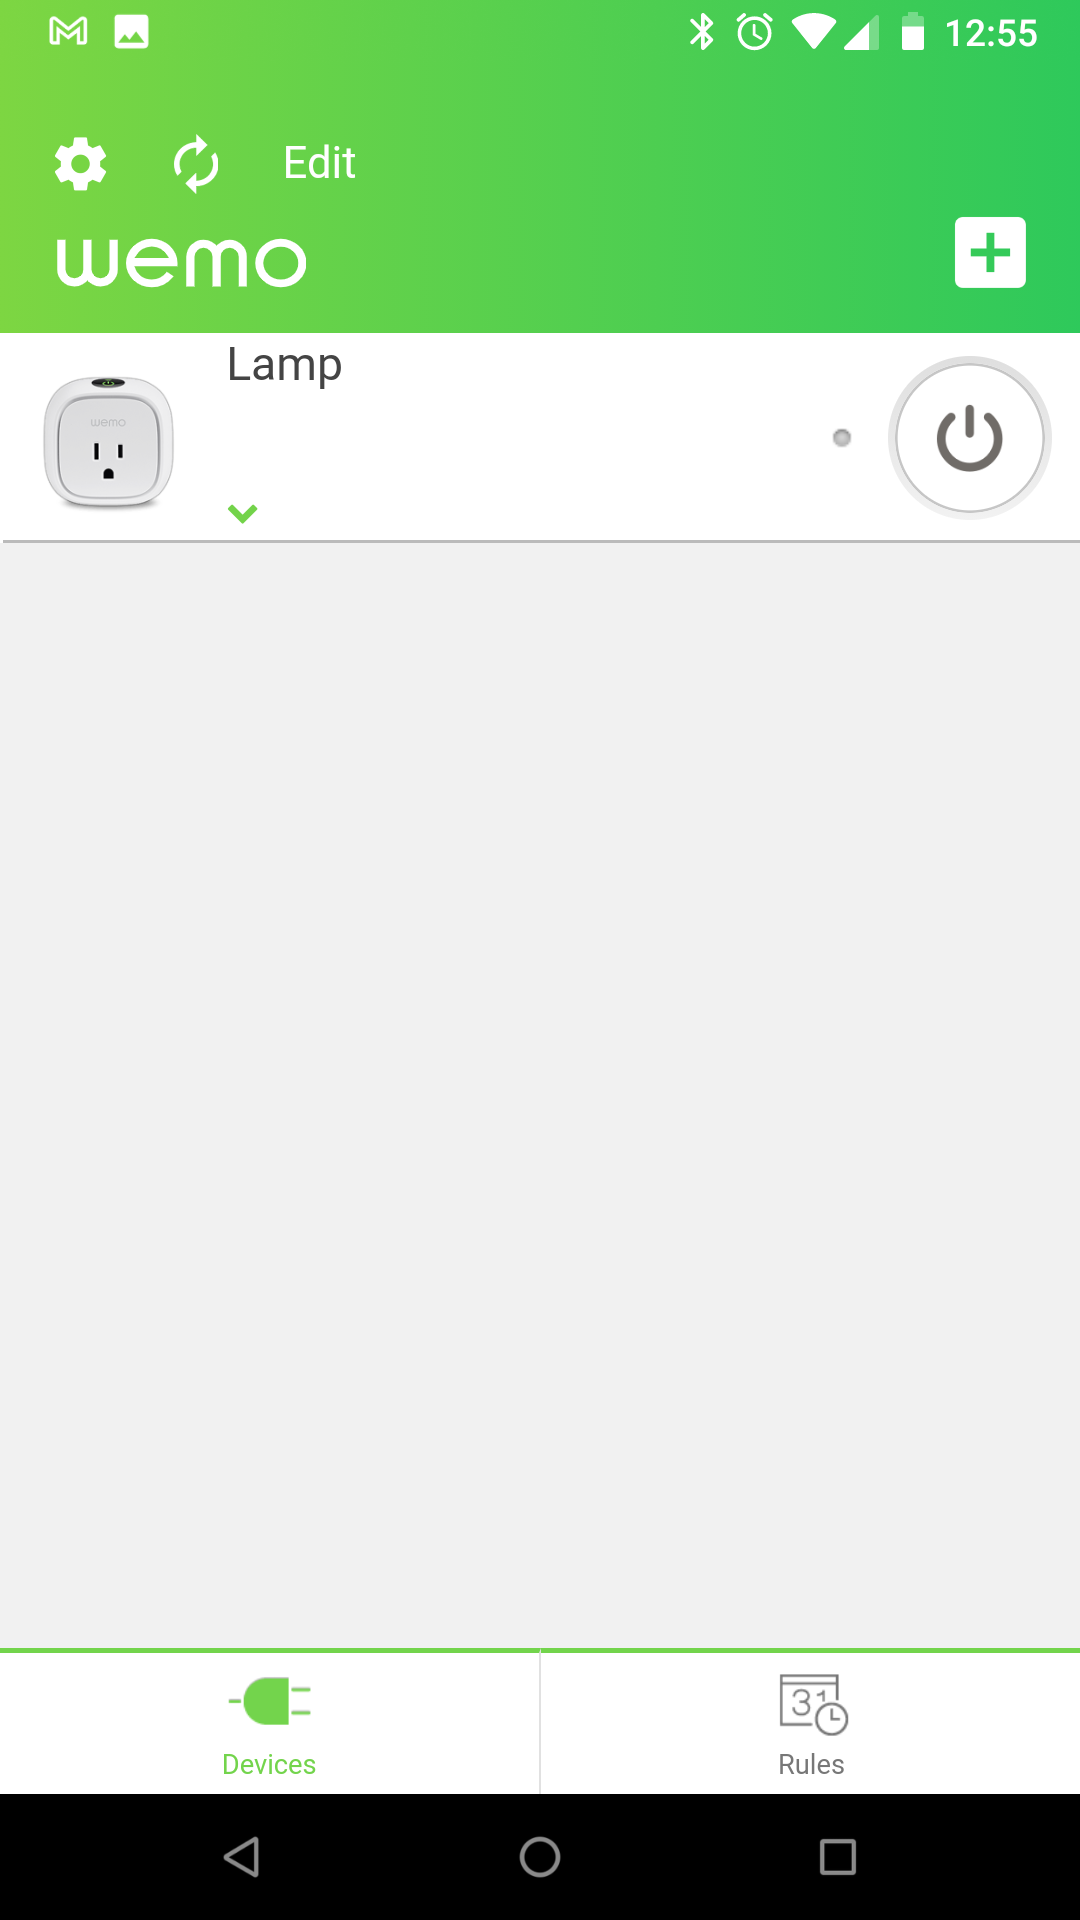
\includegraphics[scale=0.09]{figs/wemoApp/wemoAppControl.png}
\caption{Control the smart plug}
\label{fig:smartPlutControl}
\end{figure}

If any problems were encountered during the setup process, the user can go to\\
\href{https://www.wemo.com/support/}{https://www.wemo.com/support/}. Also, the paper manual provided with the WeMo box can provide additional support as it provides a comprehensive step-by-step process.